% --- FICHIER PRINCIPAL : main.tex ---

\documentclass[12pt, a4paper]{article}

% On importe toute la configuration (packages, commandes, etc.)
% depuis un fichier dédié pour plus de clarté.
% Pour gérer l'encodage des caractères, indispensable pour les accents
\usepackage[utf8]{inputenc}
% Pour la gestion de la langue française (césure, typographie, etc.)
\usepackage[french]{babel}
% Pour inclure des images
\usepackage{graphicx}
% Pour forcer le placement des figures avec [H]
\usepackage{float}
% Pour gérer les marges du document
\usepackage[top=2.5cm, bottom=2.5cm, left=2.5cm, right=2.5cm]{geometry}

\usepackage{amsmath}

% Tableaux flexibles et césure dans contenus longs
\usepackage{tabularx}
\usepackage{array}
\usepackage{seqsplit}

\usepackage{titling}

% Pour avoir des liens cliquables dans le PDF (table des matières, références)
\usepackage{hyperref}
\hypersetup{
    colorlinks=true,
    linkcolor=blue,
    filecolor=magenta,
    urlcolor=cyan,
}

% --- INFORMATIONS DU DOCUMENT ---
% Ces informations seront utilisées dans la page de garde ci-dessous
\title{Rapport de Projet : Cryptohack}
\author{Victor Bailleul \and Sébastien Leglise}
\date{\today}

% --- DÉBUT DU DOCUMENT ---
\begin{document}

% --- PAGE DE GARDE PERSONNALISÉE ---
\begin{titlepage}
    \centering % Centre tout le contenu de la page de garde

    % Espace réservé pour le logo
    \vspace*{1cm} % Espace en haut de la page
    \begin{figure}[h!]
        \centering
        % --- AJOUTEZ VOTRE LOGO ICI ---
        % Décommentez la ligne suivante et remplacez "logo.png"
        % \includegraphics[width=0.4\textwidth]{logo.png}
        
        % Si vous n'avez pas de logo, vous pouvez laisser cet espace vide
        % ou ajouter une ligne pour indiquer son emplacement.
        \fbox{Emplacement du logo} % Affiche une boîte pour visualiser l'espace
    \end{figure}
    \vspace{2cm} % Espace vertical après le logo

    % Affiche le titre en gros caractères
    {\Huge\bfseries \thetitle\par}
    \vspace{1.5cm} % Espace vertical

    % Affiche les auteurs
    {\Large \theauthor\par}
    \vspace{1cm} % Espace vertical

    % Affiche la date
    {\large \today\par}

    \vfill % Pousse le contenu restant vers le bas de la page

    % Vous pouvez ajouter le nom de votre université ou institution ici
    {\large Université Fictive de LaTeX\\ Année 2023-2024\par}
    \vspace{1cm} % Espace en bas de la page

\end{titlepage}
% --- FIN DE LA PAGE DE GARDE ---


% --- PARTIE PRÉLIMINAIRE ---
    \pagenumbering{roman} % La numérotation commence ici, sur la page 'i'
    \setcounter{page}{1}  % On force le compteur à 1 (la page sera 'i')

    \tableofcontents % La table des matières sera 'i', 'ii', etc.

% --- CORPS DU DOCUMENT ---
    \clearpage
    \pagenumbering{arabic} % On passe en chiffres arabes ET on remet le compteur à 1

% --- INCLUSION DES CHAPITRES ---
    % --- SLIDES : Introduction ---

\section{Introduction}

\begin{frame}{Contexte du projet}

    % --- Premier bloc : Plateforme CryptoHack ---
    \begin{block}{La plateforme CryptoHack}
        \begin{itemize}
            \item Plateforme d'apprentissage dédiée à la cryptographie moderne.
            \item Approche pratique : résolution de défis à difficulté croissante.
            \item Objectif : enseigner les concepts fondamentaux et avancés.
        \end{itemize}
    \end{block}

    \vspace{0.5cm}

    % --- Deuxième bloc : Intérêt des CTF ---
    \begin{alertblock}{L'intérêt des challenges de type CTF (\textit{Capture The Flag})}
        \begin{itemize}
            \item \textbf{Principe :} \textit{Gamification} de l'apprentissage en cybersécurité.
            \item \textbf{Bénéfices :}
                \begin{itemize}
                    \item Ancrage des connaissances par la pratique.
                    \item Développement de compétences techniques (analyse, résolution de problèmes).
                \end{itemize}
        \end{itemize}
    \end{alertblock}

\end{frame}

\begin{frame}
    \frametitle{Organisation du projet}
    \framesubtitle{Planification}
    \centering
    % Remplacez 'path/to/image.png' par le chemin vers votre image.
    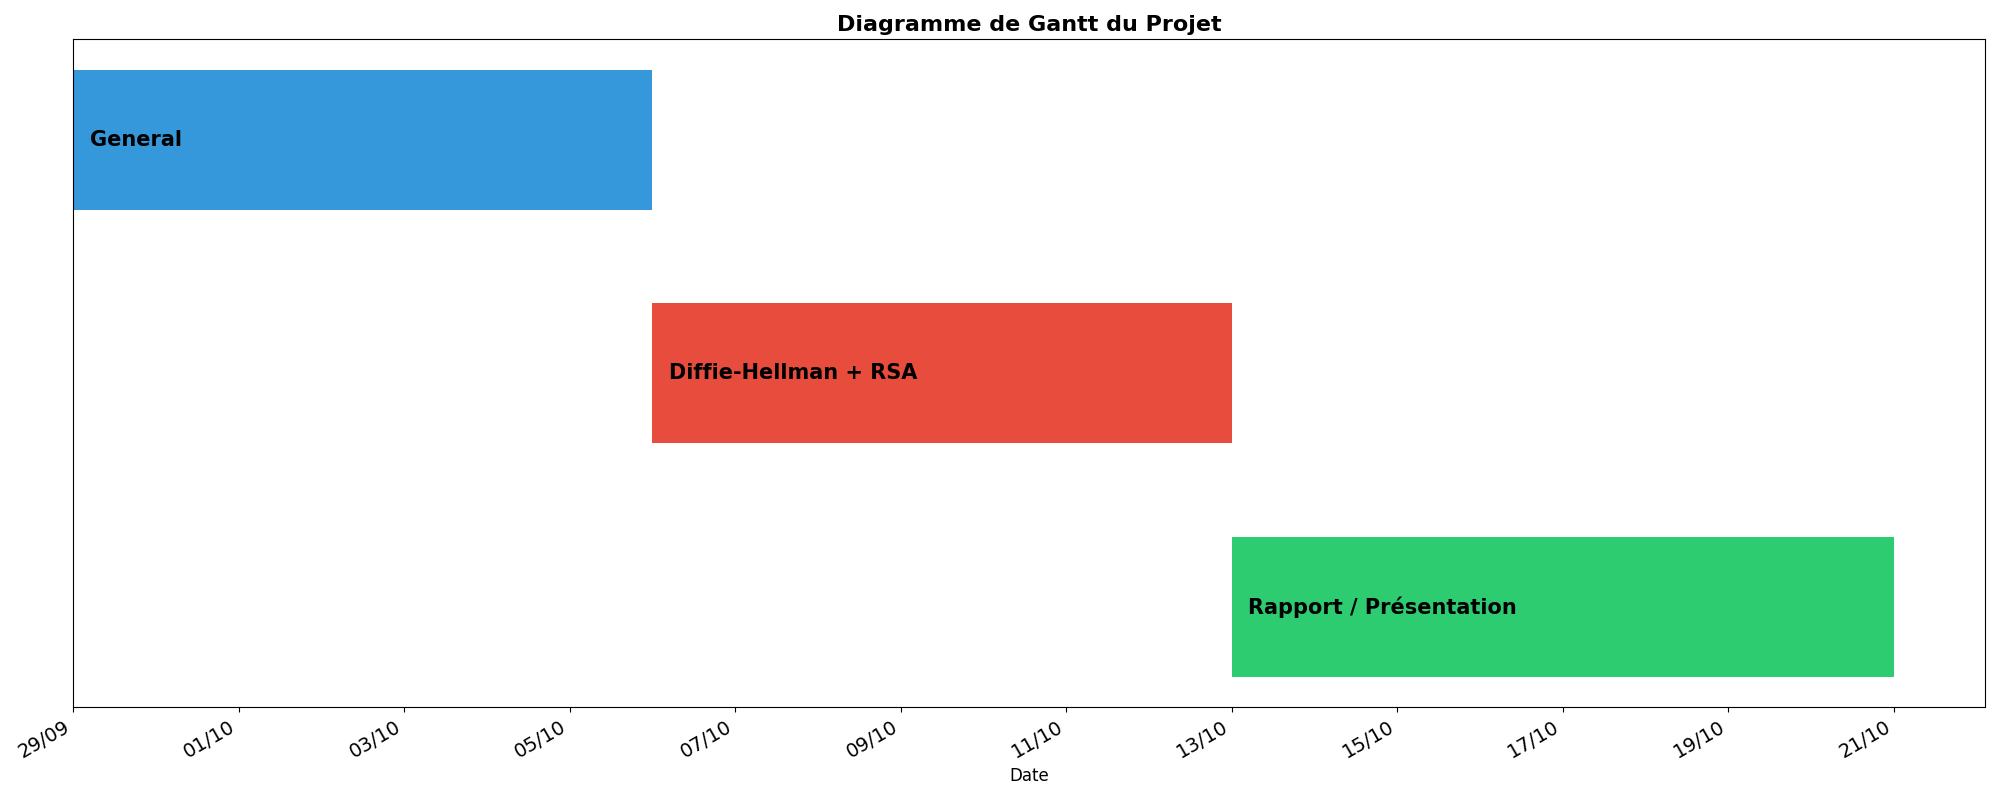
\includegraphics[width=\linewidth]{gantt.png}
\end{frame}

\begin{frame}
    \frametitle{Organisation du projet}
    \framesubtitle{Travailler en binôme}

    % --- Premier bloc : Répartition des tâches ---
    \begin{block}{Répartition des tâches individuelles}
        \centering
        \small
        \begin{tabular}{ll} 
            \textbf{} & \textit{Catégorie de challenges abordées} \\
            \textit{Victor} & General/\textbf{Encoding}, General/\textbf{XOR}, \textbf{Diffie-Hellman} \\
            \textit{Sébastien} & General/\textbf{Mathematics}, General/\textbf{Data Formats}, \textbf{RSA} \\
        \end{tabular}
    \end{block}

    \vspace{0.5cm} % Ajoute un peu d'espace entre les deux blocs

    % --- Deuxième bloc : Travail en commun ---
    \begin{alertblock}{Travail commun et collaboration}
        L'ensemble du projet a été géré via un dépôt Git partagé sur GitHub. Cette approche nous a permis de :
        \begin{itemize}
            \item \textbf{Centraliser le code} et les documents du projet.
            \item \textbf{Suivre les versions} pour éviter les conflits et les pertes de données.
            \item \textbf{Collaborer de manière asynchrone} sur les différentes parties du rapport et du code.
        \end{itemize}
    \end{alertblock}

\end{frame}
    \section{Gestion de projet (Seb)}
\subsection{Répartition du travail}
Avant de débuter les challenges \textit{CryptoHack}, nous avons planifié notre organisation en tenant compte de notre emploi du temps académique. Nous avons fixé une \textbf{date de début précise} pour disposer d'un cadre temporel clair et assurer une répartition équilibrée du travail. Une fois cette date établie, nous avons défini des \textbf{objectifs initiaux} en commençant par le module \textit{General} pour nous familiariser avec la plateforme, comprendre le format des exercices, identifier les outils nécessaires (Python, bibliothèques de cryptographie) et évaluer le niveau de difficulté.

Pour structurer notre travail, nous avons mis en place une \textbf{répartition des tâches} claire : un membre sur les modules \textit{Encoding} et \textit{XOR}, l'autre sur \textit{Mathematics} et \textit{Data Formats}. Cette division nous a permis de progresser en parallèle tout en couvrant un large spectre thématique. Nous avons également fixé une \textbf{deadline commune} pour cette phase afin de faire un point global sur l'avancement du projet. Une fois cette deadline atteinte, nous avons entamé la rédaction du rapport tout en poursuivant avec deux nouveaux modules : \textit{RSA} pour l'un et \textit{Diffie-Hellman} pour l'autre. Une nouvelle deadline a été établie pour finaliser l'ensemble du projet, incluant la complétion des derniers challenges et la rédaction définitive du rapport.

\subsection{Gestion d'un dépôt GitHub}
Dès le début du projet, nous avons créé un \textbf{dépôt GitHub partagé},
servant de point central pour le suivi et la gestion de notre travail. Ce
dépôt nous a permis d’organiser nos scripts de résolution, nos notes et les
différents fichiers associés aux challenges. L’utilisation de GitHub s’est
révélée particulièrement utile pour la \textbf{collaboration asynchrone},
notamment lorsque nos disponibilités ne coïncidaient pas.

Chaque membre disposait d’un accès complet au dépôt et pouvait le mettre à
jour dès qu’il estimait qu’une contribution était suffisamment stable ou
pertinente. Les commits étaient accompagnés de messages explicites
décrivant les modifications apportées, ce qui facilitait la compréhension
de l’évolution du projet.

\subsection{Méthodologie GitHub}
Notre utilisation de GitHub a suivi une méthodologie rigoureuse pour garantir l'efficacité de notre collaboration. Chaque solution de challenge était systématiquement organisée dans des dossiers thématiques dédiés. 

Nous avons également convenu d’un rythme de mise à jour régulier du dépôt :
chacun pouvait pousser ses modifications après vérification, en veillant à
ne pas écraser le travail de l’autre. Lorsque cela s’avérait nécessaire,
nous communiquions directement pour fusionner ou réorganiser certaines
branches, garantissant ainsi une cohérence globale dans la structure du
projet.

Une fois les premiers modules finalisés, nous avons initié la rédaction du rapport en \LaTeX{} en adoptant une structure commune pour uniformiser la présentation.  Lorsque nous avons abordé les modules \textit{RSA} et \textit{Diffie-Hellman}, nous avons restructuré notre organisation \LaTeX{} en plusieurs dossiers thématiques pour mieux classer les sections du rapport. Cette approche nous a permis de maintenir une avancée constante jusqu'à la finalisation complète du projet, en respectant les délais que nous nous étions fixés.
    \section{General}


\subsection{Encoding}

Cette première sous-partie de la catégorie General aborde les différentes
méthodes de représentation de l'information, essentielles au transport
et à l'échange de données. La maîtrise des conversions entre des formats
comme le binaire, l'hexadécimal ou le Base64 constitue un prérequis
indispensable pour aborder des défis cryptographiques plus complexes. Il
est fondamental de bien distinguer l'encodage du chiffrement : le premier
est une transformation de format, publique et réversible, qui ne vise pas
à garantir la confidentialité, contrairement au second.

Nous avons décidé de présenter le dernier challenge de cette partie,
nommé \textit{Encoding challenge}.

\subsubsection{Objectifs}
L'objectif de ce challenge consiste à développer un script pour
automatiser l'interaction avec un serveur distant de CryptoHack. Le
processus implique la réception de données encodées selon diverses
méthodes (Base64, hexadécimal, ROT13, BigInt, et UTF-8), leur décodage
approprié, puis le renvoi de la valeur décodée au serveur.

Pour valider le challenge et obtenir le flag, il est impératif d'exécuter
cette séquence de réception, décodage et renvoi avec succès cent fois
consécutives. Cette contrainte requiert une solution entièrement
automatisée, capable de gérer dynamiquement les différents types
d'encodage rencontrés.

\subsubsection{Méthode}
Le challenge met à disposition un script partiel qui présente la manière
d'envoyer et recevoir des données avec le serveur, ainsi que le script
exécuté côté serveur pour vérifier les valeurs qui lui ont été
transmises. Ces scripts nous ont permis de comprendre le format des
données transmises.

La communication avec le serveur s'effectue via l'échange d'objets au
format JSON. Pour chaque itération du challenge, le serveur envoie une
requête structurée de la manière suivante~:

\begin{verbatim}
{
    "type": "type_d_encodage",
    "encoded": "donnees_encodees"
}
\end{verbatim}

Notre script doit alors analyser cette requête, appliquer la méthode de
décodage appropriée, et renvoyer la solution au serveur sous le format
JSON attendu~:

\begin{verbatim}
{
    "decoded": "donnees_decodees"
}
\end{verbatim}

Le script côté serveur vérifie alors la validité des données décodées,
puis si cela est valide, crée un nouveau challenge. Si notre script
résout cent challenges, la prochaine requête au serveur permettra
d'afficher le \textit{flag} dans la sortie standard.

\subsubsection{Résultat}
Pour résoudre le challenge, nous nous sommes donc appuyés sur les scripts
python du challenge afin de développer un script de résolution (voir
...).

\begin{figure}[H]
    \centering
    % La commande pour insérer l'image.
    % 'width=0.8\linewidth' signifie que l'image fera 80% de la largeur du
    % texte.
    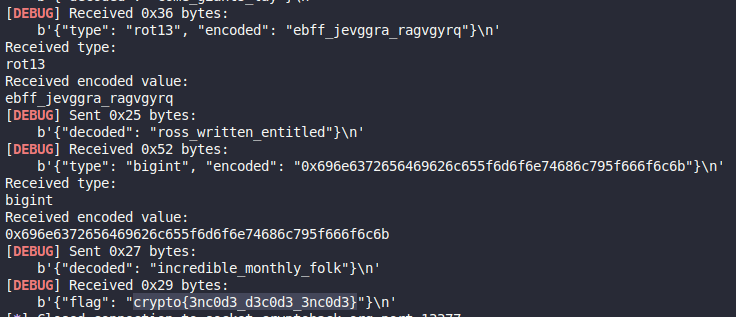
\includegraphics[width=0.8\linewidth]{Images/Encode/encode_chall_result.png}

    % La légende qui apparaîtra sous l'image.
    \caption{Ceci est le schéma explicatif de notre méthode.}

    % L'étiquette pour y faire référence plus tard.
    \label{fig:encodeChallRes}
\end{figure}

Après cent requêtes valides, le \textit{flag}
\textit{crypto\{3nc0d3\_d3c0d3\_3nc0d3\}} a été obtenu, permettant la
validation du challenge.

\subsection{Xor (Lemur)}
La deuxième sous-partie de la catégorie \textit{General} est consacrée à
l'opération XOR (ou exclusif), un concept fondamental en cryptographie
constituant l'une des briques de base de nombreux algorithmes de
chiffrement. Sa simplicité de mise en œuvre et ses propriétés
mathématiques uniques en font un outil puissant pour manipuler
l'information.

Comprendre le fonctionnement du XOR est une étape cruciale, car il se
situe à la frontière entre l'opération logique et le chiffrement. L'une
de ses propriétés essentielles est sa réversibilité: appliquer deux fois
la même clé XOR à une donnée permet de retrouver la donnée originale
($A \oplus K \oplus K = A$). Cette caractéristique est au cœur de son
utilisation dans des chiffrements à flux comme le One-Time Pad.

Nous avons décidé de présenter le challenge le plus représentatif de
cette partie, nommé \textit{Lemur XOR}.

\subsubsection{Objectifs}
Le but de ce challenge est de retrouver le \textit{flag}, à partir de
deux images fournies : \texttt{lemur.png} et \texttt{flag.png}. L'énoncé
nous apprend que ces deux images ont été chiffrées avec l'opération XOR en
utilisant la même clé secrète.

\begin{figure}[htbp] % L'environnement figure global
    \centering % Pour centrer le bloc des deux images

    \begin{minipage}{0.48\textwidth}
        \centering
        
\includegraphics[width=\linewidth]{Images/Lemur/flag.png}
        % Première image
    \end{minipage}
    \hfill % Ajoute un espace horizontal flexible entre les images
    \begin{minipage}{0.48\textwidth}
        \centering
        
\includegraphics[width=\linewidth]{Images/Lemur/lemur.png}
        % Deuxième image
    \end{minipage}

    \caption{Ceci est la légende commune pour les deux images.}
    \label{fig:deux-images}
\end{figure}

Le principe de résolution repose sur le fait qu'appliquer deux fois un XOR
avec la même clé annule l'opération. En effectuant un XOR entre les deux
images chiffrées que nous possédons, la clé secrète commune s'élimine,
ne laissant que le résultat du XOR entre les deux images originales.
C'est sur cette image combinée que le \textit{flag} devrait devenir
visible.

\subsubsection{Méthode}
Pour résoudre ce challenge, nous avons utilisé un script en Python avec la
bibliothèque de manipulation d'images \textbf{Pillow}. Nous avons commencé
par charger les deux images, \texttt{lemur.png} et \texttt{flag.png}.
Conformément aux instructions, nous avons appliqué l'opération XOR pixel
par pixel sur les valeurs de couleur RVB, et non sur les fichiers
entiers.

Nous avons donc parcouru les deux images simultanément et calculé la
nouvelle valeur de chaque pixel en effectuant un XOR sur ses composantes
rouge, verte et bleue. Nous avons ensuite utilisé ces nouveaux pixels
pour construire une image de sortie de mêmes dimensions que nous avons
sauvegardée.

\subsubsection{Résultat}
\begin{figure}[H]
    \centering
    % La commande pour insérer l'image.
    % 'width=0.8\linewidth' signifie que l'image fera 80% de la largeur du
    % texte.
    
\includegraphics[width=0.8\linewidth]{Images/Lemur/xored_result.png}

    % La légende qui apparaîtra sous l'image.
    \caption{Ceci est le schéma explicatif de notre méthode.}

    % L'étiquette pour y faire référence plus tard.
    \label{fig:encodeChallRes}
\end{figure}

\subsection{Data formats}

Le challenge s'appuie sur le principe de \emph{Certificate Transparency}
(CT), une mesure de sécurité imposée aux Autorités de Certification (CA)
pour garantir la transparence dans la délivrance des certificats TLS.

Un certificat TLS (souvent appelé certificat SSL ou certificat numérique)
est un document électronique qui remplit deux fonctions principales : il
authentifie l'identité d'un site web ou d'un domaine auprès des clients
(navigateurs, applications), et il permet d'établir une connexion
chiffrée (TLS) entre le client et le serveur, garantissant la
confidentialité et l'intégrité des données échangées.

Un \emph{CT log} est une base de données publique, append-only (où l'on ne
peut qu'ajouter des entrées) dans laquelle les certificats émis par les CA
sont enregistrés. Aujourd'hui, les principales CA doivent publier (ou
« soumettre ») chaque certificat qu'elles émettent dans au moins deux
logs CT publics pour qu'il soit accepté et reconnu comme valide par les
navigateurs modernes.

Ces logs sont audités et surveillés : chacun peut vérifier les entrées,
détecter des certificats inattendus, ou vérifier la cohérence de la
structure interne (par exemple via un arbre de Merkle) pour s'assurer
qu'on ne cache pas d'entrées.

\subsubsection{Objectifs}
L'objectif de ce challenge est double. Premièrement, il s'agit de
retrouver le sous-domaine de cryptohack.org qui utilise la même clé
publique que celle fournie dans le fichier transparency.pem dans son
certificat TLS. Deuxièmement, en visitant ce sous-domaine, il faut
obtenir le flag. À travers ce challenge, les objectifs pédagogiques sont
d'abord de comprendre le fonctionnement d’un certificat TLS et sa
structure (clé publique, signature, chaîne de confiance, etc.), ensuite
de découvrir le système des Certificate Transparency logs, qui sont des
bases de données publiques des certificats valides, puis d'apprendre à
faire correspondre une clé publique à un certificat et enfin d'utiliser
des outils d’investigation SSL/TLS et de recherche de certificats.

\subsubsection{Méthode}
Le fichier fourni est au format PEM (Privacy-Enhanced Mail), un format
standard pour les clés cryptographiques qui utilise l'encodage Base64.
La clé publique fournie était la suivante :

\begin{verbatim}
-----BEGIN PUBLIC KEY-----
MIIBIjANBgkqhkiG9w0BAQEFAAOCAQ8AMIIBCgKCAQEAuYj06m5q4M8SsEQwKX+5
NPs2lyB2k7geZw4rP68eUZmqODeqxDjv5mlLY2nz/RJsPdks4J+y5t96KAyo3S5g
mDqEOMG7JgoJ9KU+4HPQFzP9C8Gy+hisChdo9eF6UeWGTioazFDIdRUK+gZm81c1
iPEhOBIYu3Cau32LRtv+L9vzqre0Ollf7oeHqcbcMBIKL6MpsJMG+neJPnICI36B
ZZEMu6v6f8zIKuB7VUHAbDdQ6tsBzLpXz7XPBUeKPa1Fk8d22EI99peHwWt0RuJP
0QsJnsa4oj6C6lE+c5+vVHa6jVsZkpl2PuXZ05a69xORZ4oq+nwzK8O/St1hbNBX
sQIDAQAB
-----END PUBLIC KEY-----
\end{verbatim}

\paragraph{Première étape} On commence par comprendre comment relier une
empreinte SHA-256 à un certificat TLS complet et comment extraire la clé
publique d'un certificat. Un certificat TLS X.509 contient une clé
publique encapsulée et la représentation DER est la base sur laquelle on
calcule l'empreinte SHA-256 utilisée par certains services (par exemple
\texttt{crt.sh} avec le paramètre \texttt{spkisha256}). Les formats PEM
(texte Base64) et DER (binaire) sont simplement deux représentations
interchangeables de la même information.

\paragraph{Deuxième étape} La conception du script suit plusieurs
objectifs : générer l'empreinte SHA-256 de la clé publique fournie,
interroger les CT logs (par exemple via \texttt{crt.sh}) pour retrouver
les certificats correspondants, télécharger le certificat complet (PEM)
identifié dans les logs, extraire le nom de domaine du certificat,
puis accéder au sous-domaine identifié pour récupérer le flag.

\subsubsection{Résultat (Revoir présentation des resutlats)}
L'exécution du script a produit les résultats suivants :
\begin{itemize}
    \item \textbf{Empreinte (SHA-256):}
    \begin{verbatim}
    29ab37df0a4e4d252f0cf12ad854bede59038fdd9cd652cbc5c222edd26d77d2
    \end{verbatim}
    \item \textbf{Sous-domaine identifié :}
    \begin{verbatim}
    thetransparencyflagishere.cryptohack.org
    \end{verbatim}
    \item \textbf{Flag obtenu :}
    \begin{verbatim}
    crypto{thx_redpwn_for_inspiration}
    \end{verbatim}
\end{itemize}
        \section{Diffie-Hellman}
    \subsection{Introduction à l'échange de clés Diffie-Hellman}
    Cette catégorie aborde le protocole d'échange de clés de
    \textbf{Diffie-Hellman}, un mécanisme de cryptographie asymétrique.
    Proposé en 1976, il a pour objectif de résoudre le problème de la
    distribution de clés sur un canal de communication non sécurisé.

    Le principe de ce protocole repose sur l'utilisation de fonctions
    mathématiques à sens unique, dont le calcul est aisé dans une direction
    mais calculatoirement difficile à inverser. Spécifiquement, Diffie-Hellman
    s'appuie sur la difficulté du problème du \textbf{logarithme discret} dans
    un groupe fini. Ce procédé permet à deux interlocuteurs d'établir une clé
    secrète partagée sans transmission préalable de celle-ci, y compris en
    présence d'un adversaire observant la communication.

    Les challenges de cette section visent à analyser les fondements
    mathématiques de ce protocole, ainsi que les vulnérabilités pouvant
    résulter d'une implémentation incorrecte ou d'un choix de paramètres
    inadéquat.

    \subsection{L'attaque de l'homme du milieu (Man-in-the-Middle)}
    Cette sous-partie examine une vulnérabilité du protocole Diffie-Hellman~:
    l'attaque de l'homme du milieu (Man-in-the-Middle ou MitM). Le protocole de
    base, dans sa forme originelle, ne fournit aucun mécanisme d'authentification
    des interlocuteurs. Il permet de s'assurer que la clé partagée est secrète,
    mais pas de vérifier l'identité de la personne avec qui on la partage.

    Une attaque MitM exploite cette absence d'authentification. Un adversaire
    se positionne entre les deux communicants, intercepte leurs messages publics
    et établit une session Diffie-Hellman distincte avec chacun d'eux. Chaque
    interlocuteur génère alors une clé secrète partagée avec l'attaquant, tout
    en croyant communiquer directement l'un avec l'autre.

    L'adversaire peut alors déchiffrer les messages, les lire, les modifier, puis
    les rechiffrer avec la clé de l'autre session avant de les transmettre au
    destinataire final. Les challenges de cette section illustrent comment
    cette interception est mise en œuvre et comment elle compromet la
    confidentialité et l'intégrité de l'échange.

    \subsubsection{Objectifs}
    L'objectif de ce challenge est de compromettre la confidentialité d'un
    échange sécurisé par le protocole Diffie-Hellman. Le scénario repose sur
    une attaque de l'homme du milieu (Man-in-the-Middle) durant la phase de
    négociation des paramètres cryptographiques.

    La vulnérabilité exploitée est la capacité pour un attaquant d'influencer
    le choix des paramètres de groupe utilisés par les deux correspondants. En
    les contraignant à utiliser un groupe de petite taille (64 bits), le
    problème mathématique du logarithme discret, sur lequel repose la sécurité
    du protocole, devient calculatoirement soluble. La résolution de ce
    problème permet de retrouver une clé privée, et par conséquent la clé
    secrète partagée utilisée pour chiffrer la communication.

    \subsubsection{Méthode}
    Notre attaque s'est déroulée en plusieurs étapes. Premièrement, nous avons
    activement intercepté la communication initiale d'Alice, qui proposait une
    liste de groupes cryptographiques. Nous avons altéré ce message en ne
    conservant que le groupe le plus faible, caractérisé par un module de 64
    bits, avant de le transmettre à Bob. L'acceptation de cette unique option
    par Bob a été relayée à Alice, établissant ainsi un accord sur un canal de
    communication affaibli.

        \begin{figure}[H]
            \centering
            % La commande pour insérer l'image.
            % 'width=0.8\linewidth' signifie que l'image fera 80% de la largeur du
            % texte.
            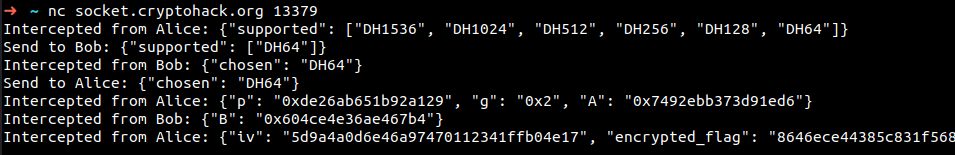
\includegraphics[width=0.9\linewidth]{Images/DiffieHellman/capture_mitm.png}

            % La légende qui apparaîtra sous l'image.
            \caption{Ceci est le schéma explicatif de notre méthode.}

            % L'étiquette pour y faire référence plus tard.
            \label{fig:mitmChallenge}
        \end{figure}

    Une fois cet accord forcé, notre rôle est devenu passif. Nous avons
    collecté les paramètres publics de l'échange : le module \texttt{p}, le
    générateur \texttt{g}, et les clés publiques d'Alice (\texttt{A}) et de
    Bob (\texttt{B}). La faible taille du module \texttt{p} a alors permis de
    résoudre le problème du logarithme discret. À l'aide d'un script Python, nous
    avons calculé la clé privée \texttt{a} d'Alice à partir des valeurs publiques
    \texttt{p}, \texttt{g} et \texttt{A}.

    La connaissance de cette clé privée nous a permis de reconstituer la clé
    secrète partagée ($s = B^a \pmod{p}$). Cette dernière a servi à dériver la
    clé de session AES, avec laquelle nous avons déchiffré le message final
    pour obtenir le \textit{flag}.

    \subsubsection{Résultat}
    L'attaque par manipulation des paramètres a réussi. En forçant l'usage d'un
    groupe faible, nous avons pu calculer la clé privée, reconstituer la clé de
    session et déchiffrer le message, révélant le \textit{flag} suivant :

    \begin{center}
        \texttt{crypto\{d0wn6r4d35\_4r3\_d4n63r0u5\}}
    \end{center}

    \subsection{Théorie des groupes}
    Cette sous-partie aborde les structures mathématiques qui sous-tendent de
    nombreux protocoles de cryptographie asymétrique~: les groupes. En
    algèbre abstraite, un \textbf{groupe} est un ensemble d'éléments muni d'une
    opération binaire qui satisfait à des axiomes spécifiques (fermeture,
    associativité, existence d'un élément neutre et d'un inverse pour chaque
    élément).

    La sécurité de protocoles comme Diffie-Hellman ne repose pas sur les
    nombres en tant que tels, mais sur les propriétés structurelles de ces
    groupes mathématiques. Des concepts comme l'ordre d'un groupe, l'ordre
    d'un élément, et la notion de \textbf{générateur} d'un \textbf{groupe
    cyclique} sont des composantes directes de l'implémentation et de
    l'analyse de sécurité de ces systèmes.

    Les challenges de cette section ont pour objectif d'étudier ces
    propriétés. Ils illustrent comment les caractéristiques d'un groupe, ou le
    choix de ses paramètres, peuvent influencer la robustesse d'un schéma
    cryptographique.

    \subsubsection{Objectifs}
    L'objectif de ce challenge est de calculer une clé secrète partagée dans une
    implémentation du protocole Diffie-Hellman utilisant un groupe additif.
    Contrairement à l'implémentation classique qui utilise un groupe
    multiplicatif d'entiers modulo un nombre premier, ce challenge transpose le
    problème dans une structure où l'opération de groupe est l'addition.

    Le principe de sécurité reste fondé sur la difficulté d'inverser une
    fonction à sens unique. Ici, l'opération équivalente à l'exponentiation est
    la multiplication scalaire. Le but est de résoudre l'équivalent du problème
    du logarithme discret dans ce contexte additif afin de retrouver une clé
    privée, puis de reconstituer la clé secrète partagée, qui constitue le
    \textit{flag}.

    \subsubsection{Méthode}
    Le challenge nous fournit les paramètres publics d'un échange
    Diffie-Hellman additif : un module premier \texttt{p}, un générateur
    \texttt{g}, ainsi que les clés publiques d'Alice (\texttt{A}) et de Bob
    (\texttt{B}). La relation qui lie la clé privée \texttt{a} à la clé
    publique \texttt{A} n'est plus $A = g^a \pmod{p}$, mais
    $A = a \cdot g \pmod{p}$.

    Le problème du logarithme discret se traduit ici par la résolution de
    l'équation $A \equiv a \cdot g \pmod{p}$ pour trouver l'inconnue
    \texttt{a}. Cette équation est une congruence linéaire qui se résout
    efficacement en calculant l'inverse modulaire de \texttt{g} modulo
    \texttt{p}. Nous avons donc déterminé la clé privée d'Alice en calculant
    $a = A \cdot g^{-1} \pmod{p}$.

    Une fois la clé privée \texttt{a} obtenue, nous avons pu calculer la clé
    secrète partagée en appliquant l'opération du groupe avec la clé publique
    de Bob. L'opération étant la multiplication scalaire, la clé secrète
    \texttt{s} est obtenue par la formule $s = a \cdot B \pmod{p}$.

    \subsubsection{Résultat}
    L'analyse de la structure de groupe additive a permis d'identifier la
    méthode de résolution appropriée. Le calcul de l'inverse modulaire nous a
    donné accès à la clé privée, menant directement à la reconstitution de la
    clé secrète partagée. Le \textit{flag} obtenu est la valeur numérique de
    cette clé secrète~:

    \begin{center}
        \texttt{crypto\{cycl1c\_6r0up\_und3r\_4dd1710n?\}}
    \end{center}

        \section{RSA}
    \subsection{Introduction au cryptosystème RSA}
    Cette catégorie aborde le cryptosystème à clé publique \textbf{RSA}, 
    décrit pour la première fois en 1977. C’est l’un des systèmes de chiffrement 
    asymétrique les plus connus et les plus utilisés dans le monde. 
    
    RSA repose sur un principe fondamental : la difficulté de factoriser de 
    grands nombres composés en leurs facteurs premiers. Cette propriété 
    mathématique permet de garantir la sécurité du système, à condition que les 
    paramètres soient choisis et implémentés correctement.
    
    Le cryptosystème RSA possède deux usages principaux. Le premier est le 
    \textbf{chiffrement}, où un utilisateur publie une clé publique permettant à 
    d’autres de lui envoyer des messages chiffrés, qu’il peut ensuite déchiffrer 
    grâce à sa clé privée. Le second est la \textbf{signature numérique}, qui 
    permet à un utilisateur de signer un message avec sa clé privée, afin que 
    quiconque puisse vérifier l’authenticité et l’intégrité du message à l’aide 
    de la clé publique correspondante.
    
    Les challenges de cette section ont pour objectif d’explorer les fondements 
    du cryptosystème RSA, tout en mettant en évidence les erreurs courantes et 
    les failles d’implémentation qui ont, dans certains cas, conduit à des 
    attaques réelles causant des pertes financières considérables.

    \subsection{RSA Multi-Factor Attack}
    Le challenge \texttt{"ManyPrime"} propose un fichier contenant un module RSA $n$, un exposant public $e$ et un ciphertext $ct$. L'énoncé contient deux indices explicites : l'auteur indique qu'il utilisera "over 30" facteurs premiers et renvoie vers la méthode des courbes elliptiques (ECM). Ces indications orientent la stratégie d'attaque : extraire un grand nombre de facteurs premiers relativement petits grace à l'ECM, et retrouver la clef privée pour déchiffrer le message.
    
    \subsubsection{Objectifs}
    L'objectif est donc de récupérer le flag contenu dans le ciphertext. Concrètement, il faut factoriser \textbf{n} en l'ensemble de ses facteurs premiers. Puis calculer $d = e^{-1} \pmod{\varphi(n)}$ où $\varphi(n)=\prod_i (p_i-1)$ et finalement déchiffrer $\mathrm{ct}$ pour obtenir le plaintext (le flag). 
    
    \subsubsection{Méthode}
    \paragraph{Principe de l'attaque}
    La vulnérabilité exploitée dans ce scénario réside dans une conception cryptographique déficiente : la construction d'un module RSA comme produit d'un grand nombre de facteurs premiers de petite taille. Cette approche, bien que contre-intuitive, affaiblit considérablement la résistance du module aux algorithmes de factorisation modernes. En effet, les méthodes de factorisation telles qu'ECM (Elliptic Curve Method) deviennent particulièrement efficaces lorsque le plus grand facteur premier n'excède pas une certaine taille critique.
    
    \paragraph{Mise en œuvre pratique}
    La première étape consiste à configurer l'environnement de calcul en initialisant un environnement Python virtuel et en installant les bibliothèques spécialisées nécessaires. La bibliothèque \texttt{primefac} fournit l'implémentation de l'algorithme ECM, tandis que \texttt{pycryptodome} offre les primitives cryptographiques essentielles pour les opérations arithmétiques modulaires.
    
    Le processus de factorisation proprement dit s'articule autour d'une boucle itérative. Initialement, une variable temporaire \texttt{current} reçoit la valeur du module $n$ à factoriser. À chaque itération, tant que \texttt{current} demeure composite, l'algorithme ECM est invoqué via \texttt{primefac.ecm()} pour en extraire un facteur premier $p$. Ce facteur est immédiatement ajouté à une liste de facteurs reconnus, tandis que \texttt{current} est mis à jour par division entière par $p$. Une vérification systématique de la primalité du résidu guide la progression du processus.
    
    \paragraph{Reconstruction et déchiffrement}
    Une fois la factorisation complétée, une phase de validation est entreprise. L'intégrité de la décomposition est vérifiée en recalculant le produit de tous les facteurs identifiés, qui doit restituer exactement la valeur originale $n$. La fonction indicatrice d'Euler est alors calculée selon la relation $\varphi(n) = \prod (p_i - 1)$ pour l'ensemble des facteurs premiers $p_i$.
    
    L'exposant privé $d$ est déterminé comme solution de l'équation $e \cdot d \equiv 1 \pmod{\varphi(n)}$ via l'algorithme d'Euclide étendu. Finalement, le message chiffré $ct$ est déchiffré par exponentiation modulaire selon la transformation $pt = ct^d \pmod{n}$, restaurant ainsi le message original.
    
    Cette méthodologie démontre l'importance cruciale d'utiliser des modules RSA composés de deux facteurs premiers de grande taille en pratique cryptographique.
        
    \subsubsection{Résultat}
   Le script extrait plusieurs facteurs premiers et les affiche sur le terminal. Les valeurs obtenues sont présentées dans le tableau ci-dessous :

    \begin{table}[h!]
    \centering
    \begin{tabular}{lll}
      $p_1 = 17281246625998849649$ & $p_2 = 9389357739583927789$ & $p_3 = 10638241655447339831$ \\
      $p_4 = 16656402470578844539$ & $p_5 = 14100640260554622013$ & $p_6 = 9303850685953812323$ \\
      $p_7 = 17174065872156629921$ & $p_8 = 14963354250199553339$ & $\dots$ \\
    \end{tabular}
    \caption{Facteurs premiers extraits par ECM}
    \label{tab:facteurs}
    \end{table}
    
    Après les calculs de vérification et de déchiffrement, on obtient le message en clair suivant :
    
    \begin{center}
    \texttt{crypto\{700\_m4ny\_5m4ll\_f4c70r5\}}
    \end{center}



    \subsection{Cryptanalyse RSA avec exposant faible}
    Cette sous-partie présente l'analyse du challenge « Vote for Pedro » qui illustre une vulnérabilité cryptographique classique dans l'implémentation du chiffrement RSA. Le challenge met en avant les dangers liés à l'utilisation d'un exposant public faible, particulièrement lorsque combiné avec des messages de petite taille et l'absence de mécanisme de padding approprié. La résolution de ce challenge démontre comment il est possible de forger des signatures sans disposer de la clé privée, compromettant ainsi l'intégrité du système d'authentification.
    
    \subsubsection{Objectifs}
    L'objectif principal de ce challenge consiste à obtenir un flag en votant pour Pedro avec une signature valide émise par Alice. Le serveur vérifie la signature du vote en utilisant la clé publique d'Alice et retourne le flag uniquement si le message déchiffré correspond exactement à la chaîne « VOTE FOR PEDRO ». La difficulté réside dans l'impossibilité d'accéder à la clé privée d'Alice pour signer le message légitimement.
    
    \subsubsection{Méthode}
    Le challenge fournit deux éléments essentiels : le script du serveur et la clé publique d'Alice. L'analyse du script serveur révèle le mécanisme de vérification des signatures. Le serveur reçoit un vote signé sous forme hexadécimale, applique la vérification RSA en calculant le vote à la puissance de l'exposant public modulo $N$, puis convertit le résultat en bytes. Le message est ensuite extrait en prenant la partie suivant le dernier octet nul avant d'être comparé avec la chaîne attendue.

    La clé publique d'Alice présente une particularité cruciale : l'exposant public $e = 3$. Cette valeur faible, combinée avec l'absence de padding robuste, crée une vulnérabilité exploitable en permettant une attaque par extraction de racine cubique. En effet, lorsque le message original est inférieur à la racine cubique de $N$, l'opération de signature peut être inversée sans recours au modulo, rendant possible la forge de signature.
    
    \paragraph{Principe mathématique}
    Le système vérifie la signature via l'équation RSA standard $\text{vote}^e \pmod{N}$. Avec $e = 3$ et un message $M$ suffisamment petit ($M < \sqrt[3]{N}$), l'opération modulo devient inutile, simplifiant l'équation en $\text{vote}^3 = M$. La signature s'obtient donc par calcul direct de $\sqrt[3]{M}$.
    
    Le message « VOTE FOR PEDRO » n'étant pas un cube parfait, on cherche un entier $S$ tel que $S^3$ partage les mêmes bits de poids faible que le message original. Cette condition est suffisante car le serveur extrait le message après le dernier octet nul, ignorant les bits de poids fort.
 
    \paragraph{Algorithme de résolution}
    L'algorithme \texttt{cube\_root\_2\_pow} calcule la racine cubique bit par bit. Initialisé avec $s = c \pmod{8}$ pour capturer les trois bits de poids faible, il procède par raffinement successif. Pour chaque position $k$, il ajuste le bit correspondant pour minimiser la différence entre $s^3$ et $c$ modulo $2^k$, garantissant la convergence vers la solution optimale.
    
    \paragraph{Implémentation technique}
    L'implémentation établit une connexion socket, convertit le message en entier via \texttt{bytes\_to\_long}, et calcule la racine cubique avec une précision adaptée. La signature résultante est convertie en hexadécimal et transmise dans un payload JSON conforme au protocole attendu par le serveur.
   
    \subsubsection{Résultat}
    L'exécution du script de résolution produit le résultat suivant après connexion au serveur :

    \begin{verbatim}
    Place your vote. Pedro offers a reward to anyone who votes for him!
    {"flag": "crypto{y0ur_v0t3_i5_my_v0t3}"}
    \end{verbatim}


    % --- SLIDES : Conclusion ---

\section{Conclusion}

\begin{frame}{Bilan du projet}
    \begin{itemize}
        \item Compétences acquises.
        \item Difficultés rencontrées.
        \item Perspectives et suite possible.
    \end{itemize}
\end{frame}

\begin{frame}
    \centering
    \Huge{\bfseries Questions ?}
\end{frame}

% --- ANNEXES ---
    \appendix
    \newpage
    \section*{Annexes}
    \addcontentsline{toc}{section}{Annexes}

    % --- FICHIER : Annexes/annexes.tex ---

\section{Script de résolution du challenge Encoding}
\label{annexe:script-encoding}

Voici le code Python complet utilisé pour le challenge "Encoding".

% Pour du code, il est recommandé d'utiliser le package "listings"
\begin{verbatim}
import pwn
import json

# ... (le reste de votre code) ...
\end{verbatim}

\section{Script de résolution du challenge Lemur XOR}
\label{annexe:script-lemur}

Voici le code utilisé pour le challenge "Lemur XOR".

\begin{verbatim}
from PIL import Image

# ... (le reste de votre code) ...
\end{verbatim}


\section{Script de résolution du challenge Transparency}
\label{annexe:script-transparency}

Voici le code utilisé pour le challenge "Transparency".

\begin{verbatim}
#!/usr/bin/env python3

from Crypto.PublicKey import RSA
from OpenSSL.crypto import load_certificate, FILETYPE_PEM
import hashlib
import json
import requests

f = open("transparency_afff0345c6f99bf80eab5895458d8eab.pem")
key = RSA.import_key(f.read()).public_key()

sha256 = hashlib.sha256(key.exportKey(format="DER"))
fp = sha256.hexdigest()
print("fingerprint:", fp)

user_agent = 'Mozilla/5.0 (Windows NT 6.1; WOW64; rv:40.0) Gecko/20100101 Firefox/40.1'
url = "https://crt.sh/?spkisha256={hash}&output=json"

req = requests.get(url.format(hash=fp), headers={'User-Agent': user_agent})
content = req.content.decode('utf-8')
data = json.loads(content)
id = data[0]["id"]
download_url = "https://crt.sh/?d={id}"
req = requests.get(download_url.format(id=id), headers={'User-Agent': user_agent})
PEMcert = req.content.decode('utf-8')

cert = load_certificate(FILETYPE_PEM, PEMcert) 
CN = cert.get_subject().commonName 
print("Nom du domaine: ", CN)

flag_url = "https://" + CN
req = requests.get(flag_url, headers={'User-Agent': user_agent})
flag = req.content.decode('utf-8')
print("Flag:", flag)
\end{verbatim}


\section{Script de résolution du challenge Manyprime}
\label{annexe:script-Manyprime}

Voici le code utilisé pour le challenge "Manyprime".

\begin{verbatim}
#!/usr/bin/env python3

from Crypto.Util.number import inverse, long_to_bytes
import primefac
import math

n = ...
e = 65537
ct = ...

factors = []
current = n

while current > 1:
    if primefac.isprime(current):
        factors.append(current)
        break
    else:
        p = primefac.ecm(current)
        print(f"p:{p}")
        factors.append(p)
        current //= p

product = 1
for p in factors:
    product *= p
assert n == product

phi = 1
for p in factors:
    phi *= (p - 1)

d = inverse(e, phi)
pt = pow(ct, d, n)
decrypted = long_to_bytes(pt)
print(decrypted)
\end{verbatim}

\section{Script de résolution du challenge Vote for Pedro}
\label{annexe:script-vote-for-pedro}


\begin{verbatim}
#!/usr/bin/env python3

from Crypto.Util.number import bytes_to_long, long_to_bytes
import socket
import json

host = 'socket.cryptohack.org'
port = 13375

N = ...

e = 3

sock = socket.socket(socket.AF_INET, socket.SOCK_STREAM)
sock.connect((host, port))
data = sock.recv(1024)
print(data)

T = b'VOTE FOR PEDRO'
c = bytes_to_long(T)

def cube_root_2_pow(c, k_max):
    s = c % 8
    for k in range(3, k_max):
        diff = s**3 - c
        d = diff // (2**k)
        t = (-d) % 2
        s = s + t * (2**k)
    return s

s = cube_root_2_pow(c, len(T)*8 + 8)
sign_hex = long_to_bytes(s).hex()

payload = {
    "option": "vote",
    "vote": sign_hex
}

sock.send(json.dumps(payload).encode())
flag = sock.recv(1024)
print(flag)
\end{verbatim}


\end{document}